\section{Further SAE Latent Analysis}\label{app:further_analysis}

\begin{figure*}[htbp]
    \centering
    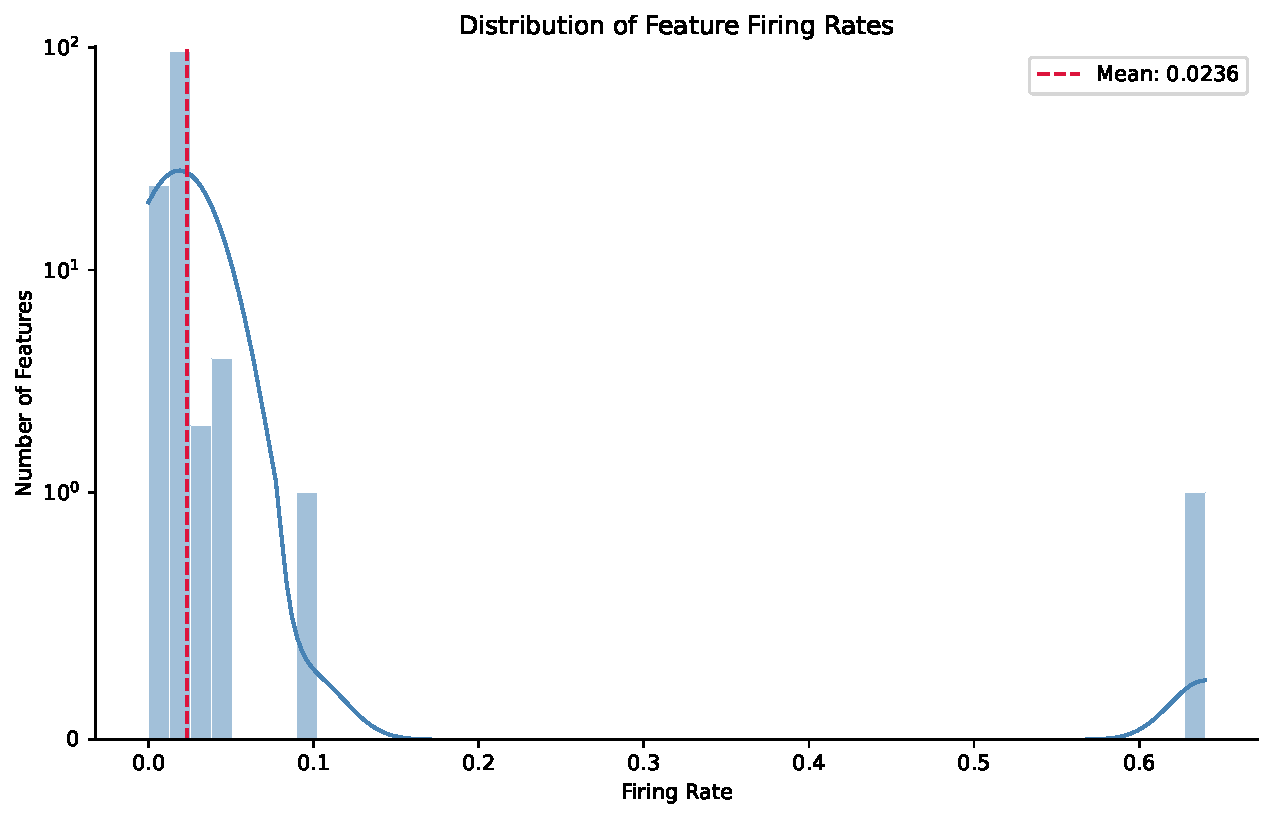
\includegraphics[width=0.7\linewidth]{figures/firing_rate_histogram.pdf}
    \caption{
        This histogram shows the distribution of firing rates for the SAE checkpoint's latents. The y-axis uses a symmetric logarithmic scale with a linear scale between $[-1, 1]$.
        A given latent's firing rate is the proportion of inputs which cause that latent to activate.
        The special latents are the only ones with a firing rate greater than one standard deviation from the mean (mean: 0.0236, standard deviation: 0.0559): latent 11 has rate 0.6400, latent 56 has rate 0.0991.
        }
    \label{fig:firing_rate_histogram}
\end{figure*} 

\begin{figure*}[htbp]
    \centering
    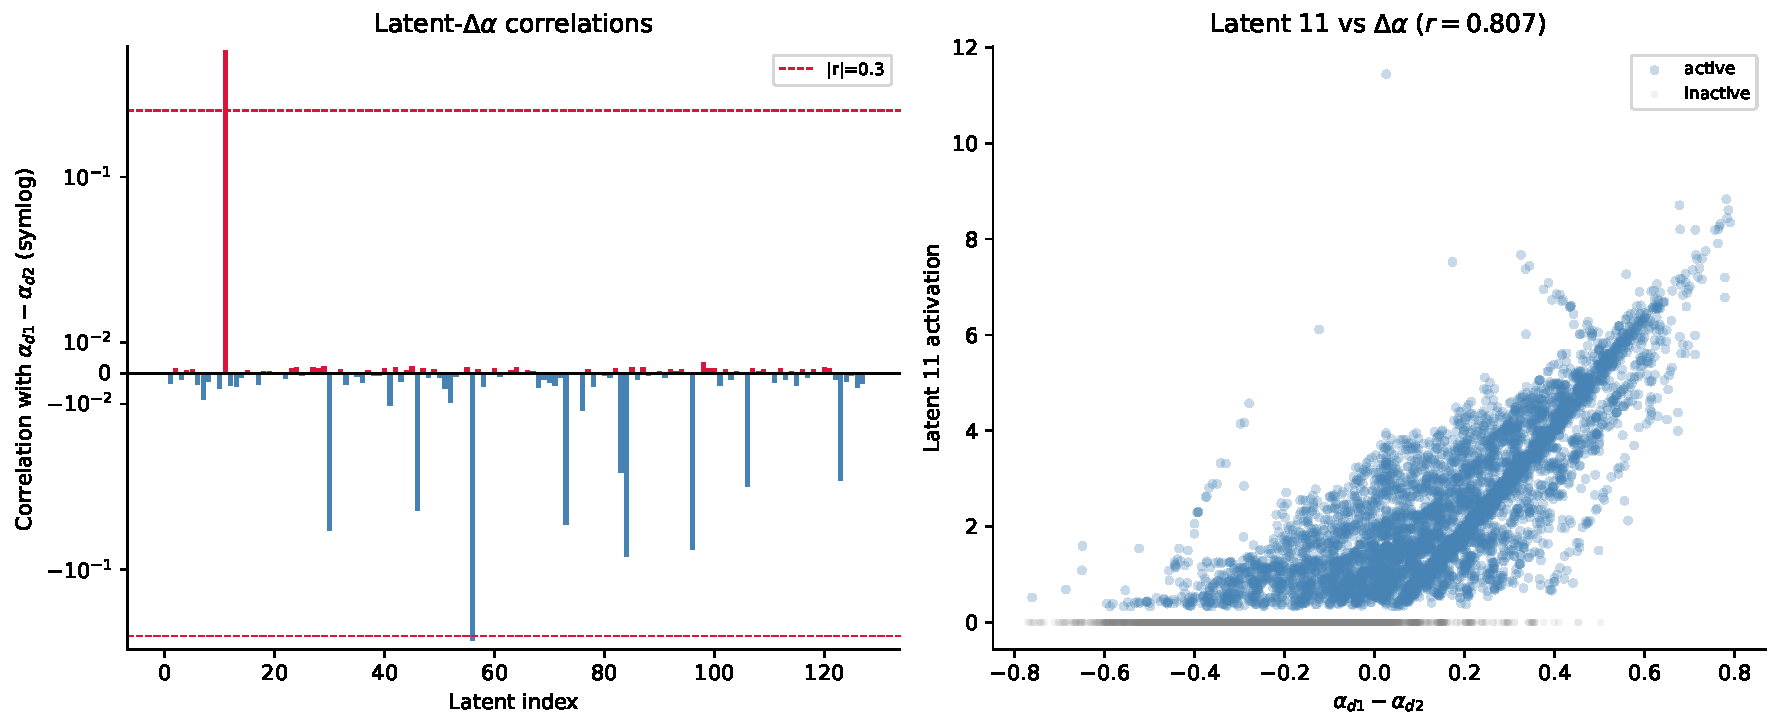
\includegraphics[width=\linewidth]{figures/alpha_diff_correlation_plot.pdf}
    \caption{
        \textbf{Left}: This plot shows the (Pearson) correlation of each latent with \(\Delta \alpha = \alpha_{s \to d_1} - \alpha_{s \to d_2}\), which is intuitively the emphasis given to $d_1$ over $d_2$ by \texttt{SEP} in the transformer model's first layer's attention pattern. The y-axis uses a symmetric logarithmic scale with a linear scale between $[-0.05,0.05]$. $d_1$-favouring latents are highlighted red and $d_2$-favouring latents are highlighted blue. The top three strongest correlations are: latent 11 with $r=0.807$, latent 56 with $r=-0.3213$, and latent 96 with $r=0.0036$.
        \textbf{Right}: This plot shows the correlation of latent 11 with $\Delta \alpha$ in more detail, as this latent has the strongest correlation. All 10,000 possible input bigrams are plotted, and highlighted blue if they activate latent 11 and grey otherwise. We see that the latent activates with greater magnitude for larger $\Delta \alpha$.
        }
    \label{fig:alpha_diff_correlation_plot}
\end{figure*} 

% TODO
% blabla

% However, in JumpReLU test we find a latent that activates more than the specials but doesnt seem to be a special (no alpha\_diff corr or scaling)